
% Default to the notebook output style

    


% Inherit from the specified cell style.




    
\documentclass[11pt]{article}

    
    
    \usepackage[T1]{fontenc}
    % Nicer default font (+ math font) than Computer Modern for most use cases
    \usepackage{mathpazo}

    % Basic figure setup, for now with no caption control since it's done
    % automatically by Pandoc (which extracts ![](path) syntax from Markdown).
    \usepackage{graphicx}
    % We will generate all images so they have a width \maxwidth. This means
    % that they will get their normal width if they fit onto the page, but
    % are scaled down if they would overflow the margins.
    \makeatletter
    \def\maxwidth{\ifdim\Gin@nat@width>\linewidth\linewidth
    \else\Gin@nat@width\fi}
    \makeatother
    \let\Oldincludegraphics\includegraphics
    % Set max figure width to be 80% of text width, for now hardcoded.
    \renewcommand{\includegraphics}[1]{\Oldincludegraphics[width=.8\maxwidth]{#1}}
    % Ensure that by default, figures have no caption (until we provide a
    % proper Figure object with a Caption API and a way to capture that
    % in the conversion process - todo).
    \usepackage{caption}
    \DeclareCaptionLabelFormat{nolabel}{}
    \captionsetup{labelformat=nolabel}

    \usepackage{adjustbox} % Used to constrain images to a maximum size 
    \usepackage{xcolor} % Allow colors to be defined
    \usepackage{enumerate} % Needed for markdown enumerations to work
    \usepackage{geometry} % Used to adjust the document margins
    \usepackage{amsmath} % Equations
    \usepackage{amssymb} % Equations
    \usepackage{textcomp} % defines textquotesingle
    % Hack from http://tex.stackexchange.com/a/47451/13684:
    \AtBeginDocument{%
        \def\PYZsq{\textquotesingle}% Upright quotes in Pygmentized code
    }
    \usepackage{upquote} % Upright quotes for verbatim code
    \usepackage{eurosym} % defines \euro
    \usepackage[mathletters]{ucs} % Extended unicode (utf-8) support
    \usepackage[utf8x]{inputenc} % Allow utf-8 characters in the tex document
    \usepackage{fancyvrb} % verbatim replacement that allows latex
    \usepackage{grffile} % extends the file name processing of package graphics 
                         % to support a larger range 
    % The hyperref package gives us a pdf with properly built
    % internal navigation ('pdf bookmarks' for the table of contents,
    % internal cross-reference links, web links for URLs, etc.)
    \usepackage{hyperref}
    \usepackage{longtable} % longtable support required by pandoc >1.10
    \usepackage{booktabs}  % table support for pandoc > 1.12.2
    \usepackage[inline]{enumitem} % IRkernel/repr support (it uses the enumerate* environment)
    \usepackage[normalem]{ulem} % ulem is needed to support strikethroughs (\sout)
                                % normalem makes italics be italics, not underlines
    

    
    
    % Colors for the hyperref package
    \definecolor{urlcolor}{rgb}{0,.145,.698}
    \definecolor{linkcolor}{rgb}{.71,0.21,0.01}
    \definecolor{citecolor}{rgb}{.12,.54,.11}

    % ANSI colors
    \definecolor{ansi-black}{HTML}{3E424D}
    \definecolor{ansi-black-intense}{HTML}{282C36}
    \definecolor{ansi-red}{HTML}{E75C58}
    \definecolor{ansi-red-intense}{HTML}{B22B31}
    \definecolor{ansi-green}{HTML}{00A250}
    \definecolor{ansi-green-intense}{HTML}{007427}
    \definecolor{ansi-yellow}{HTML}{DDB62B}
    \definecolor{ansi-yellow-intense}{HTML}{B27D12}
    \definecolor{ansi-blue}{HTML}{208FFB}
    \definecolor{ansi-blue-intense}{HTML}{0065CA}
    \definecolor{ansi-magenta}{HTML}{D160C4}
    \definecolor{ansi-magenta-intense}{HTML}{A03196}
    \definecolor{ansi-cyan}{HTML}{60C6C8}
    \definecolor{ansi-cyan-intense}{HTML}{258F8F}
    \definecolor{ansi-white}{HTML}{C5C1B4}
    \definecolor{ansi-white-intense}{HTML}{A1A6B2}

    % commands and environments needed by pandoc snippets
    % extracted from the output of `pandoc -s`
    \providecommand{\tightlist}{%
      \setlength{\itemsep}{0pt}\setlength{\parskip}{0pt}}
    \DefineVerbatimEnvironment{Highlighting}{Verbatim}{commandchars=\\\{\}}
    % Add ',fontsize=\small' for more characters per line
    \newenvironment{Shaded}{}{}
    \newcommand{\KeywordTok}[1]{\textcolor[rgb]{0.00,0.44,0.13}{\textbf{{#1}}}}
    \newcommand{\DataTypeTok}[1]{\textcolor[rgb]{0.56,0.13,0.00}{{#1}}}
    \newcommand{\DecValTok}[1]{\textcolor[rgb]{0.25,0.63,0.44}{{#1}}}
    \newcommand{\BaseNTok}[1]{\textcolor[rgb]{0.25,0.63,0.44}{{#1}}}
    \newcommand{\FloatTok}[1]{\textcolor[rgb]{0.25,0.63,0.44}{{#1}}}
    \newcommand{\CharTok}[1]{\textcolor[rgb]{0.25,0.44,0.63}{{#1}}}
    \newcommand{\StringTok}[1]{\textcolor[rgb]{0.25,0.44,0.63}{{#1}}}
    \newcommand{\CommentTok}[1]{\textcolor[rgb]{0.38,0.63,0.69}{\textit{{#1}}}}
    \newcommand{\OtherTok}[1]{\textcolor[rgb]{0.00,0.44,0.13}{{#1}}}
    \newcommand{\AlertTok}[1]{\textcolor[rgb]{1.00,0.00,0.00}{\textbf{{#1}}}}
    \newcommand{\FunctionTok}[1]{\textcolor[rgb]{0.02,0.16,0.49}{{#1}}}
    \newcommand{\RegionMarkerTok}[1]{{#1}}
    \newcommand{\ErrorTok}[1]{\textcolor[rgb]{1.00,0.00,0.00}{\textbf{{#1}}}}
    \newcommand{\NormalTok}[1]{{#1}}
    
    % Additional commands for more recent versions of Pandoc
    \newcommand{\ConstantTok}[1]{\textcolor[rgb]{0.53,0.00,0.00}{{#1}}}
    \newcommand{\SpecialCharTok}[1]{\textcolor[rgb]{0.25,0.44,0.63}{{#1}}}
    \newcommand{\VerbatimStringTok}[1]{\textcolor[rgb]{0.25,0.44,0.63}{{#1}}}
    \newcommand{\SpecialStringTok}[1]{\textcolor[rgb]{0.73,0.40,0.53}{{#1}}}
    \newcommand{\ImportTok}[1]{{#1}}
    \newcommand{\DocumentationTok}[1]{\textcolor[rgb]{0.73,0.13,0.13}{\textit{{#1}}}}
    \newcommand{\AnnotationTok}[1]{\textcolor[rgb]{0.38,0.63,0.69}{\textbf{\textit{{#1}}}}}
    \newcommand{\CommentVarTok}[1]{\textcolor[rgb]{0.38,0.63,0.69}{\textbf{\textit{{#1}}}}}
    \newcommand{\VariableTok}[1]{\textcolor[rgb]{0.10,0.09,0.49}{{#1}}}
    \newcommand{\ControlFlowTok}[1]{\textcolor[rgb]{0.00,0.44,0.13}{\textbf{{#1}}}}
    \newcommand{\OperatorTok}[1]{\textcolor[rgb]{0.40,0.40,0.40}{{#1}}}
    \newcommand{\BuiltInTok}[1]{{#1}}
    \newcommand{\ExtensionTok}[1]{{#1}}
    \newcommand{\PreprocessorTok}[1]{\textcolor[rgb]{0.74,0.48,0.00}{{#1}}}
    \newcommand{\AttributeTok}[1]{\textcolor[rgb]{0.49,0.56,0.16}{{#1}}}
    \newcommand{\InformationTok}[1]{\textcolor[rgb]{0.38,0.63,0.69}{\textbf{\textit{{#1}}}}}
    \newcommand{\WarningTok}[1]{\textcolor[rgb]{0.38,0.63,0.69}{\textbf{\textit{{#1}}}}}
    
    
    % Define a nice break command that doesn't care if a line doesn't already
    % exist.
    \def\br{\hspace*{\fill} \\* }
    % Math Jax compatability definitions
    \def\gt{>}
    \def\lt{<}
    % Document parameters
    \title{index}
    
    
    

    % Pygments definitions
    
\makeatletter
\def\PY@reset{\let\PY@it=\relax \let\PY@bf=\relax%
    \let\PY@ul=\relax \let\PY@tc=\relax%
    \let\PY@bc=\relax \let\PY@ff=\relax}
\def\PY@tok#1{\csname PY@tok@#1\endcsname}
\def\PY@toks#1+{\ifx\relax#1\empty\else%
    \PY@tok{#1}\expandafter\PY@toks\fi}
\def\PY@do#1{\PY@bc{\PY@tc{\PY@ul{%
    \PY@it{\PY@bf{\PY@ff{#1}}}}}}}
\def\PY#1#2{\PY@reset\PY@toks#1+\relax+\PY@do{#2}}

\expandafter\def\csname PY@tok@ch\endcsname{\let\PY@it=\textit\def\PY@tc##1{\textcolor[rgb]{0.25,0.50,0.50}{##1}}}
\expandafter\def\csname PY@tok@kp\endcsname{\def\PY@tc##1{\textcolor[rgb]{0.00,0.50,0.00}{##1}}}
\expandafter\def\csname PY@tok@sc\endcsname{\def\PY@tc##1{\textcolor[rgb]{0.73,0.13,0.13}{##1}}}
\expandafter\def\csname PY@tok@gt\endcsname{\def\PY@tc##1{\textcolor[rgb]{0.00,0.27,0.87}{##1}}}
\expandafter\def\csname PY@tok@kd\endcsname{\let\PY@bf=\textbf\def\PY@tc##1{\textcolor[rgb]{0.00,0.50,0.00}{##1}}}
\expandafter\def\csname PY@tok@kr\endcsname{\let\PY@bf=\textbf\def\PY@tc##1{\textcolor[rgb]{0.00,0.50,0.00}{##1}}}
\expandafter\def\csname PY@tok@nl\endcsname{\def\PY@tc##1{\textcolor[rgb]{0.63,0.63,0.00}{##1}}}
\expandafter\def\csname PY@tok@sr\endcsname{\def\PY@tc##1{\textcolor[rgb]{0.73,0.40,0.53}{##1}}}
\expandafter\def\csname PY@tok@kt\endcsname{\def\PY@tc##1{\textcolor[rgb]{0.69,0.00,0.25}{##1}}}
\expandafter\def\csname PY@tok@se\endcsname{\let\PY@bf=\textbf\def\PY@tc##1{\textcolor[rgb]{0.73,0.40,0.13}{##1}}}
\expandafter\def\csname PY@tok@vc\endcsname{\def\PY@tc##1{\textcolor[rgb]{0.10,0.09,0.49}{##1}}}
\expandafter\def\csname PY@tok@nc\endcsname{\let\PY@bf=\textbf\def\PY@tc##1{\textcolor[rgb]{0.00,0.00,1.00}{##1}}}
\expandafter\def\csname PY@tok@s\endcsname{\def\PY@tc##1{\textcolor[rgb]{0.73,0.13,0.13}{##1}}}
\expandafter\def\csname PY@tok@fm\endcsname{\def\PY@tc##1{\textcolor[rgb]{0.00,0.00,1.00}{##1}}}
\expandafter\def\csname PY@tok@mo\endcsname{\def\PY@tc##1{\textcolor[rgb]{0.40,0.40,0.40}{##1}}}
\expandafter\def\csname PY@tok@vi\endcsname{\def\PY@tc##1{\textcolor[rgb]{0.10,0.09,0.49}{##1}}}
\expandafter\def\csname PY@tok@ge\endcsname{\let\PY@it=\textit}
\expandafter\def\csname PY@tok@s2\endcsname{\def\PY@tc##1{\textcolor[rgb]{0.73,0.13,0.13}{##1}}}
\expandafter\def\csname PY@tok@vg\endcsname{\def\PY@tc##1{\textcolor[rgb]{0.10,0.09,0.49}{##1}}}
\expandafter\def\csname PY@tok@cp\endcsname{\def\PY@tc##1{\textcolor[rgb]{0.74,0.48,0.00}{##1}}}
\expandafter\def\csname PY@tok@kn\endcsname{\let\PY@bf=\textbf\def\PY@tc##1{\textcolor[rgb]{0.00,0.50,0.00}{##1}}}
\expandafter\def\csname PY@tok@kc\endcsname{\let\PY@bf=\textbf\def\PY@tc##1{\textcolor[rgb]{0.00,0.50,0.00}{##1}}}
\expandafter\def\csname PY@tok@gp\endcsname{\let\PY@bf=\textbf\def\PY@tc##1{\textcolor[rgb]{0.00,0.00,0.50}{##1}}}
\expandafter\def\csname PY@tok@gr\endcsname{\def\PY@tc##1{\textcolor[rgb]{1.00,0.00,0.00}{##1}}}
\expandafter\def\csname PY@tok@ss\endcsname{\def\PY@tc##1{\textcolor[rgb]{0.10,0.09,0.49}{##1}}}
\expandafter\def\csname PY@tok@sb\endcsname{\def\PY@tc##1{\textcolor[rgb]{0.73,0.13,0.13}{##1}}}
\expandafter\def\csname PY@tok@dl\endcsname{\def\PY@tc##1{\textcolor[rgb]{0.73,0.13,0.13}{##1}}}
\expandafter\def\csname PY@tok@il\endcsname{\def\PY@tc##1{\textcolor[rgb]{0.40,0.40,0.40}{##1}}}
\expandafter\def\csname PY@tok@gi\endcsname{\def\PY@tc##1{\textcolor[rgb]{0.00,0.63,0.00}{##1}}}
\expandafter\def\csname PY@tok@nn\endcsname{\let\PY@bf=\textbf\def\PY@tc##1{\textcolor[rgb]{0.00,0.00,1.00}{##1}}}
\expandafter\def\csname PY@tok@c1\endcsname{\let\PY@it=\textit\def\PY@tc##1{\textcolor[rgb]{0.25,0.50,0.50}{##1}}}
\expandafter\def\csname PY@tok@nf\endcsname{\def\PY@tc##1{\textcolor[rgb]{0.00,0.00,1.00}{##1}}}
\expandafter\def\csname PY@tok@vm\endcsname{\def\PY@tc##1{\textcolor[rgb]{0.10,0.09,0.49}{##1}}}
\expandafter\def\csname PY@tok@gd\endcsname{\def\PY@tc##1{\textcolor[rgb]{0.63,0.00,0.00}{##1}}}
\expandafter\def\csname PY@tok@w\endcsname{\def\PY@tc##1{\textcolor[rgb]{0.73,0.73,0.73}{##1}}}
\expandafter\def\csname PY@tok@gs\endcsname{\let\PY@bf=\textbf}
\expandafter\def\csname PY@tok@ow\endcsname{\let\PY@bf=\textbf\def\PY@tc##1{\textcolor[rgb]{0.67,0.13,1.00}{##1}}}
\expandafter\def\csname PY@tok@c\endcsname{\let\PY@it=\textit\def\PY@tc##1{\textcolor[rgb]{0.25,0.50,0.50}{##1}}}
\expandafter\def\csname PY@tok@cpf\endcsname{\let\PY@it=\textit\def\PY@tc##1{\textcolor[rgb]{0.25,0.50,0.50}{##1}}}
\expandafter\def\csname PY@tok@err\endcsname{\def\PY@bc##1{\setlength{\fboxsep}{0pt}\fcolorbox[rgb]{1.00,0.00,0.00}{1,1,1}{\strut ##1}}}
\expandafter\def\csname PY@tok@gu\endcsname{\let\PY@bf=\textbf\def\PY@tc##1{\textcolor[rgb]{0.50,0.00,0.50}{##1}}}
\expandafter\def\csname PY@tok@nt\endcsname{\let\PY@bf=\textbf\def\PY@tc##1{\textcolor[rgb]{0.00,0.50,0.00}{##1}}}
\expandafter\def\csname PY@tok@sa\endcsname{\def\PY@tc##1{\textcolor[rgb]{0.73,0.13,0.13}{##1}}}
\expandafter\def\csname PY@tok@na\endcsname{\def\PY@tc##1{\textcolor[rgb]{0.49,0.56,0.16}{##1}}}
\expandafter\def\csname PY@tok@ni\endcsname{\let\PY@bf=\textbf\def\PY@tc##1{\textcolor[rgb]{0.60,0.60,0.60}{##1}}}
\expandafter\def\csname PY@tok@mb\endcsname{\def\PY@tc##1{\textcolor[rgb]{0.40,0.40,0.40}{##1}}}
\expandafter\def\csname PY@tok@si\endcsname{\let\PY@bf=\textbf\def\PY@tc##1{\textcolor[rgb]{0.73,0.40,0.53}{##1}}}
\expandafter\def\csname PY@tok@cs\endcsname{\let\PY@it=\textit\def\PY@tc##1{\textcolor[rgb]{0.25,0.50,0.50}{##1}}}
\expandafter\def\csname PY@tok@bp\endcsname{\def\PY@tc##1{\textcolor[rgb]{0.00,0.50,0.00}{##1}}}
\expandafter\def\csname PY@tok@sx\endcsname{\def\PY@tc##1{\textcolor[rgb]{0.00,0.50,0.00}{##1}}}
\expandafter\def\csname PY@tok@gh\endcsname{\let\PY@bf=\textbf\def\PY@tc##1{\textcolor[rgb]{0.00,0.00,0.50}{##1}}}
\expandafter\def\csname PY@tok@mi\endcsname{\def\PY@tc##1{\textcolor[rgb]{0.40,0.40,0.40}{##1}}}
\expandafter\def\csname PY@tok@sd\endcsname{\let\PY@it=\textit\def\PY@tc##1{\textcolor[rgb]{0.73,0.13,0.13}{##1}}}
\expandafter\def\csname PY@tok@m\endcsname{\def\PY@tc##1{\textcolor[rgb]{0.40,0.40,0.40}{##1}}}
\expandafter\def\csname PY@tok@sh\endcsname{\def\PY@tc##1{\textcolor[rgb]{0.73,0.13,0.13}{##1}}}
\expandafter\def\csname PY@tok@k\endcsname{\let\PY@bf=\textbf\def\PY@tc##1{\textcolor[rgb]{0.00,0.50,0.00}{##1}}}
\expandafter\def\csname PY@tok@o\endcsname{\def\PY@tc##1{\textcolor[rgb]{0.40,0.40,0.40}{##1}}}
\expandafter\def\csname PY@tok@mh\endcsname{\def\PY@tc##1{\textcolor[rgb]{0.40,0.40,0.40}{##1}}}
\expandafter\def\csname PY@tok@nv\endcsname{\def\PY@tc##1{\textcolor[rgb]{0.10,0.09,0.49}{##1}}}
\expandafter\def\csname PY@tok@no\endcsname{\def\PY@tc##1{\textcolor[rgb]{0.53,0.00,0.00}{##1}}}
\expandafter\def\csname PY@tok@mf\endcsname{\def\PY@tc##1{\textcolor[rgb]{0.40,0.40,0.40}{##1}}}
\expandafter\def\csname PY@tok@s1\endcsname{\def\PY@tc##1{\textcolor[rgb]{0.73,0.13,0.13}{##1}}}
\expandafter\def\csname PY@tok@cm\endcsname{\let\PY@it=\textit\def\PY@tc##1{\textcolor[rgb]{0.25,0.50,0.50}{##1}}}
\expandafter\def\csname PY@tok@nb\endcsname{\def\PY@tc##1{\textcolor[rgb]{0.00,0.50,0.00}{##1}}}
\expandafter\def\csname PY@tok@ne\endcsname{\let\PY@bf=\textbf\def\PY@tc##1{\textcolor[rgb]{0.82,0.25,0.23}{##1}}}
\expandafter\def\csname PY@tok@go\endcsname{\def\PY@tc##1{\textcolor[rgb]{0.53,0.53,0.53}{##1}}}
\expandafter\def\csname PY@tok@nd\endcsname{\def\PY@tc##1{\textcolor[rgb]{0.67,0.13,1.00}{##1}}}

\def\PYZbs{\char`\\}
\def\PYZus{\char`\_}
\def\PYZob{\char`\{}
\def\PYZcb{\char`\}}
\def\PYZca{\char`\^}
\def\PYZam{\char`\&}
\def\PYZlt{\char`\<}
\def\PYZgt{\char`\>}
\def\PYZsh{\char`\#}
\def\PYZpc{\char`\%}
\def\PYZdl{\char`\$}
\def\PYZhy{\char`\-}
\def\PYZsq{\char`\'}
\def\PYZdq{\char`\"}
\def\PYZti{\char`\~}
% for compatibility with earlier versions
\def\PYZat{@}
\def\PYZlb{[}
\def\PYZrb{]}
\makeatother


    % Exact colors from NB
    \definecolor{incolor}{rgb}{0.0, 0.0, 0.5}
    \definecolor{outcolor}{rgb}{0.545, 0.0, 0.0}



    
    % Prevent overflowing lines due to hard-to-break entities
    \sloppy 
    % Setup hyperref package
    \hypersetup{
      breaklinks=true,  % so long urls are correctly broken across lines
      colorlinks=true,
      urlcolor=urlcolor,
      linkcolor=linkcolor,
      citecolor=citecolor,
      }
    % Slightly bigger margins than the latex defaults
    
    \geometry{verbose,tmargin=1in,bmargin=1in,lmargin=1in,rmargin=1in}
    
    

    \begin{document}
    
    
    \maketitle
    
    

    
    \begin{Verbatim}[commandchars=\\\{\}]
{\color{incolor}In [{\color{incolor}7}]:} \PY{k+kn}{import} \PY{n+nn}{os}\PY{o}{,} \PY{n+nn}{sys}
        
        \PY{c+c1}{\PYZsh{}figure display}
        \PY{k+kn}{from} \PY{n+nn}{IPython}\PY{n+nn}{.}\PY{n+nn}{core}\PY{n+nn}{.}\PY{n+nn}{display} \PY{k}{import} \PY{n}{HTML}
        \PY{k+kn}{from} \PY{n+nn}{IPython}\PY{n+nn}{.}\PY{n+nn}{display} \PY{k}{import} \PY{n}{display}\PY{p}{,} \PY{n}{IFrame}
        
        \PY{c+c1}{\PYZsh{}files for data munging}
        \PY{n}{file\PYZus{}dir} \PY{o}{=} \PY{n}{os}\PY{o}{.}\PY{n}{getcwd}\PY{p}{(}\PY{p}{)}
        \PY{n}{sys}\PY{o}{.}\PY{n}{path}\PY{o}{.}\PY{n}{append}\PY{p}{(}\PY{n}{file\PYZus{}dir} \PY{o}{+} \PY{l+s+s2}{\PYZdq{}}\PY{l+s+s2}{/scripts}\PY{l+s+s2}{\PYZdq{}}\PY{p}{)}
        
        \PY{c+c1}{\PYZsh{}inline plotting}
        \PY{k+kn}{from} \PY{n+nn}{bokeh}\PY{n+nn}{.}\PY{n+nn}{resources} \PY{k}{import} \PY{n}{INLINE}
        
        \PY{c+c1}{\PYZsh{}set size of figures}
        \PY{k+kn}{from} \PY{n+nn}{notebook}\PY{n+nn}{.}\PY{n+nn}{services}\PY{n+nn}{.}\PY{n+nn}{config} \PY{k}{import} \PY{n}{ConfigManager}
        \PY{n}{cm} \PY{o}{=} \PY{n}{ConfigManager}\PY{p}{(}\PY{p}{)}
        \PY{n}{cm}\PY{o}{.}\PY{n}{update}\PY{p}{(}\PY{l+s+s1}{\PYZsq{}}\PY{l+s+s1}{livereveal}\PY{l+s+s1}{\PYZsq{}}\PY{p}{,} \PY{p}{\PYZob{}}
                  \PY{l+s+s1}{\PYZsq{}}\PY{l+s+s1}{width}\PY{l+s+s1}{\PYZsq{}}\PY{p}{:} \PY{l+m+mi}{1500}\PY{p}{,}
                  \PY{l+s+s1}{\PYZsq{}}\PY{l+s+s1}{height}\PY{l+s+s1}{\PYZsq{}}\PY{p}{:} \PY{l+m+mi}{1000}\PY{p}{,}
        \PY{p}{\PYZcb{}}\PY{p}{)}
\end{Verbatim}


\begin{Verbatim}[commandchars=\\\{\}]
{\color{outcolor}Out[{\color{outcolor}7}]:} \{'height': 1000, 'width': 1500\}
\end{Verbatim}
            
    \begin{Verbatim}[commandchars=\\\{\}]
{\color{incolor}In [{\color{incolor}104}]:} \PY{k+kn}{import} \PY{n+nn}{os}
          \PY{k+kn}{from} \PY{n+nn}{IPython}\PY{n+nn}{.}\PY{n+nn}{display} \PY{k}{import} \PY{n}{IFrame}
          \PY{k+kn}{import} \PY{n+nn}{pandas} \PY{k}{as} \PY{n+nn}{pd}
\end{Verbatim}


    \begin{Verbatim}[commandchars=\\\{\}]
{\color{incolor}In [{\color{incolor}114}]:} \PYZpc{}\PYZpc{}bash 
          jupyter nbconvert \PYZti{}/Documents/Projects/RSS\PYZhy{}2018/index.ipynb \PYZhy{}\PYZhy{}to slides \PYZhy{}\PYZhy{}post serve
\end{Verbatim}


    \begin{Verbatim}[commandchars=\\\{\}]
Process is terminated.

    \end{Verbatim}

    \begin{Verbatim}[commandchars=\\\{\}]
{\color{incolor}In [{\color{incolor} }]:} \PYZpc{}\PYZpc{}bash 
        jupyter nbconvert \PYZti{}/Documents/Projects/RSS\PYZhy{}2018/index.ipynb \PYZhy{}\PYZhy{}to slides
\end{Verbatim}


    \section{Traffic flow as an early indicator for GDP
growth}\label{traffic-flow-as-an-early-indicator-for-gdp-growth}

\textbf{Edward Rowland}\\
Big Data - Methodology

\textbf{Jessica Lawrence, Nathan Davis, Anthony Fitzroy and Ben Vince}\\
Data Engineering - DaaS

\textbf{Duncan Elliot}\\
Time series analysis - Methodology

Office for National Statistics, UK

    \begin{Verbatim}[commandchars=\\\{\}]
{\color{incolor}In [{\color{incolor}21}]:} \PY{c+c1}{\PYZsh{} source: https://stackoverflow.com/questions/27934885/how\PYZhy{}to\PYZhy{}hide\PYZhy{}code\PYZhy{}from\PYZhy{}cells\PYZhy{}in\PYZhy{}ipython\PYZhy{}notebook\PYZhy{}visualized\PYZhy{}with\PYZhy{}nbviewer}
         
         \PY{n}{HTML}\PY{p}{(}\PY{l+s+s1}{\PYZsq{}\PYZsq{}\PYZsq{}}\PY{l+s+s1}{\PYZlt{}script\PYZgt{}}
         \PY{l+s+s1}{code\PYZus{}show=true; }
         \PY{l+s+s1}{function code\PYZus{}toggle() }\PY{l+s+s1}{\PYZob{}}
         \PY{l+s+s1}{ if (code\PYZus{}show)}\PY{l+s+s1}{\PYZob{}}
         \PY{l+s+s1}{ \PYZdl{}(}\PY{l+s+s1}{\PYZsq{}}\PY{l+s+s1}{div.input}\PY{l+s+s1}{\PYZsq{}}\PY{l+s+s1}{).hide();}
         \PY{l+s+s1}{ \PYZcb{} else }\PY{l+s+s1}{\PYZob{}}
         \PY{l+s+s1}{ \PYZdl{}(}\PY{l+s+s1}{\PYZsq{}}\PY{l+s+s1}{div.input}\PY{l+s+s1}{\PYZsq{}}\PY{l+s+s1}{).show();}
         \PY{l+s+s1}{ \PYZcb{}}
         \PY{l+s+s1}{ code\PYZus{}show = !code\PYZus{}show}
         \PY{l+s+s1}{\PYZcb{} }
         \PY{l+s+s1}{\PYZdl{}( document ).ready(code\PYZus{}toggle);}
         \PY{l+s+s1}{\PYZlt{}/script\PYZgt{}}
         \PY{l+s+s1}{\PYZlt{}form action=}\PY{l+s+s1}{\PYZdq{}}\PY{l+s+s1}{javascript:code\PYZus{}toggle()}\PY{l+s+s1}{\PYZdq{}}\PY{l+s+s1}{\PYZgt{}\PYZlt{}input type=}\PY{l+s+s1}{\PYZdq{}}\PY{l+s+s1}{submit}\PY{l+s+s1}{\PYZdq{}}\PY{l+s+s1}{ value=}\PY{l+s+s1}{\PYZdq{}}\PY{l+s+s1}{Click here to toggle on/off the raw code.}\PY{l+s+s1}{\PYZdq{}}\PY{l+s+s1}{\PYZgt{}\PYZlt{}/form\PYZgt{}}\PY{l+s+s1}{\PYZsq{}\PYZsq{}\PYZsq{}}\PY{p}{)}
\end{Verbatim}


\begin{Verbatim}[commandchars=\\\{\}]
{\color{outcolor}Out[{\color{outcolor}21}]:} <IPython.core.display.HTML object>
\end{Verbatim}
            
    \begin{Verbatim}[commandchars=\\\{\}]
{\color{incolor}In [{\color{incolor}1}]:} \PY{c+c1}{\PYZsh{}source: https://stackoverflow.com/questions/9031783/hide\PYZhy{}all\PYZhy{}warnings\PYZhy{}in\PYZhy{}ipython}
        \PY{k+kn}{from} \PY{n+nn}{IPython}\PY{n+nn}{.}\PY{n+nn}{display} \PY{k}{import} \PY{n}{HTML}
        
        \PY{n}{HTML}\PY{p}{(}\PY{l+s+s1}{\PYZsq{}\PYZsq{}\PYZsq{}}\PY{l+s+s1}{\PYZlt{}script\PYZgt{}}
        \PY{l+s+s1}{code\PYZus{}show\PYZus{}err=false; }
        \PY{l+s+s1}{function code\PYZus{}toggle\PYZus{}err() }\PY{l+s+s1}{\PYZob{}}
        \PY{l+s+s1}{ if (code\PYZus{}show\PYZus{}err)}\PY{l+s+s1}{\PYZob{}}
        \PY{l+s+s1}{ \PYZdl{}(}\PY{l+s+s1}{\PYZsq{}}\PY{l+s+s1}{div.output\PYZus{}stderr}\PY{l+s+s1}{\PYZsq{}}\PY{l+s+s1}{).hide();}
        \PY{l+s+s1}{ \PYZcb{} else }\PY{l+s+s1}{\PYZob{}}
        \PY{l+s+s1}{ \PYZdl{}(}\PY{l+s+s1}{\PYZsq{}}\PY{l+s+s1}{div.output\PYZus{}stderr}\PY{l+s+s1}{\PYZsq{}}\PY{l+s+s1}{).show();}
        \PY{l+s+s1}{ \PYZcb{}}
        \PY{l+s+s1}{ code\PYZus{}show\PYZus{}err = !code\PYZus{}show\PYZus{}err}
        \PY{l+s+s1}{\PYZcb{} }
        \PY{l+s+s1}{\PYZdl{}( document ).ready(code\PYZus{}toggle\PYZus{}err);}
        \PY{l+s+s1}{\PYZlt{}/script\PYZgt{}}
        
        \PY{l+s+s1}{\PYZlt{}form action=}\PY{l+s+s1}{\PYZdq{}}\PY{l+s+s1}{javascript:code\PYZus{}toggle\PYZus{}err()}\PY{l+s+s1}{\PYZdq{}}\PY{l+s+s1}{\PYZgt{}\PYZlt{}input type=}\PY{l+s+s1}{\PYZdq{}}\PY{l+s+s1}{submit}\PY{l+s+s1}{\PYZdq{}}\PY{l+s+s1}{ value=}\PY{l+s+s1}{\PYZdq{}}\PY{l+s+s1}{Click here to toggle on/off warnings.}\PY{l+s+s1}{\PYZdq{}}\PY{l+s+s1}{\PYZgt{}\PYZlt{}/form\PYZgt{}}\PY{l+s+s1}{\PYZsq{}\PYZsq{}\PYZsq{}}\PY{p}{)}
\end{Verbatim}


\begin{Verbatim}[commandchars=\\\{\}]
{\color{outcolor}Out[{\color{outcolor}1}]:} <IPython.core.display.HTML object>
\end{Verbatim}
            
    \section{Talk Structure}\label{talk-structure}

\begin{enumerate}
\def\labelenumi{\arabic{enumi}.}
\tightlist
\item
  Background
\item
  Other research
\item
  High Frequency traffic counts
\item
  Supervised learning models
\item
  Discussion
\end{enumerate}

\textbf{Other things I may not have time to talk about but are in these
slides} 7. Future direction with some more time series analysis 8.
Correlations and time series models with annual data 9. Trends and
seasonal decomposition of daily traffic counts

    Background

    \subsubsection{Traffic flow is thought to be elastic to a number of
economic
factors}\label{traffic-flow-is-thought-to-be-elastic-to-a-number-of-economic-factors}

\begin{itemize}
\tightlist
\item
  GDP: More stuff being made that needs to be moved about
\item
  Salary: More money means people might travel more for work, business
  and leisure
\item
  Employment: More people in work may mean more commuting
\item
  Inflation: If the cost of living goes up, that might mean less traffic
  as people cut back on expenses
\end{itemize}

    \subsubsection{How is this useful?}\label{how-is-this-useful}

    \textbf{1. More localised estimates}\\
Identify areas of low or negative growth that would be lost if looking
at the national figures

    \textbf{2. Potential early indicator}\\
A recession is defined as having two or more quarters of negative GDP
growth. The UK won't officially know if it is in recession until around
6-7 months after it started.

    \textbf{3. Identify impacts of specific events}\\
With high frequency data, it could identify the impacts of events
(Weather, terrorist attacks, Brexit etc.)

    \textbf{This aim is to find relationships between traffic and economic
indicators to see if this could work}

    \section{Other work}\label{other-work}

    \subsubsection{Stats Netherlands}\label{stats-netherlands}

Research using data from an extensive road sensor network in The
Netherlands shows correlations with traffic flow and a number of
economic measures with a lag of 3 months

\begin{longtable}[c]{@{}lcr@{}}
\toprule
Measure & Total Traffic & Cat 1 (\textless{} 5.6m)
Traffic\tabularnewline
\midrule
\endhead
Inflation & -0.42 & -0.43\tabularnewline
Unemployment & -0.47 & -0.41\tabularnewline
Income & 0.74 & 0.74\tabularnewline
GDP & 0.54 & 0.63\tabularnewline
\bottomrule
\end{longtable}

    \begin{itemize}
\tightlist
\item
  Income followed by GDP look to be the strongest correlates
\item
  Larger vehicles (HGVs) correlate most strongly with GDP
\item
  Perhaps some weaker correlations with inflation and Unemployment
\end{itemize}

    Killan, Ros, "Road Traffic Correlations with Economic Variables: The Big
Data Perspective., 2017,
https://pdfs.semanticscholar.org/1f1d/b563d229bdd4fd8c90ad8dd6c5cd3487f76b.pdf

    \subsubsection{Statistical Office of the Republic of Slovenia
(SURS)}\label{statistical-office-of-the-republic-of-slovenia-surs}

    \begin{itemize}
\tightlist
\item
  Used traffic flow to estimate GDP figure 45 days before its
  publication.
\item
  PCA with linear regression to estimate GDP
\item
  Found that cargo vehicles were the best predictor of GDP, within 1\%
  of the GDP figure
\end{itemize}

    Črt Grahonja, 2018, Use of alternative data sources as flash estimates
of economic indicators, European conference on quality in official
statistics June 2018:
https://www.q2018.pl/papers-presentations/?drawer=Sessions*Session\%2022

    \subsection{Statistics Finland}\label{statistics-finland}

    \begin{itemize}
\tightlist
\item
  Uses Company level data and traffic loops to produce two nowcasts and
  a 16-day backcast of GDP
\item
  Reduce factors by two-step PCA and shrinkage step
\item
  16 day backcast was as accurate as the first estimate of GDP when
  comparing both to the revised figure
\item
  Traffic flow and company data were similar when estimating GDP
\end{itemize}

    Henri Luomaranta, 2018, Nowcasting Finnish Real Economic Activity: a
Machine Learning Approach, European conference on Quality in official
statistics June 2018:
https://www.q2018.pl/papers-presentations/?drawer=Sessions*Session\%2022

    \section{High frequency traffic flow
data}\label{high-frequency-traffic-flow-data}

    \subsection{Highways England data}\label{highways-england-data}

    Highways England provides an open dataset containing traffic flow counts
at 15 minute intervals for Motorways and major A-Roads across England.

\begin{itemize}
\tightlist
\item
  The Data Engineering team in DaaS have scraped and ingested this data

  \begin{itemize}
  \tightlist
  \item
    Over 2 million seperate files
  \item
    Over 200Gb of data
  \item
    Seperates out small (\textless{} 5.6m), medium (5.6 - 6.6m), large
    (6.6 - 11.6m) and very large (\textgreater{} 11.6m) vehicles
  \end{itemize}
\item
  Really exciting high frequency dataset - ideally suited for this work

  \begin{itemize}
  \tightlist
  \item
    Look at the approaches used in Slovenia and Finland
  \item
    Previously we have replicated correlations found by Stats
    Netherlands using annual data
  \end{itemize}
\end{itemize}

    \subsubsection{Data processing}\label{data-processing}

    Make the data manageable - Aggregate to give mean traffic count for a 15
minute period across the UK for each day - Created features by
decomposing the data to find trend and yearly seasonal components as
well as moving averages - For supervised learning, create a feature for
each traffic variable for each day in time period - Compare this to
quarterly GDP

    \section{Modelling}\label{modelling}

    A range of different approaches were used including...

\begin{itemize}
\tightlist
\item
  SARIMAX - with a variety of different quarterly weighted average
  traffic flow measures as exogenous regressors
\item
  PCA for decomposition and linear regression with and without shrinkage
  methods
\item
  PCA for decomposition and Random Forest Regression
\item
  3-fold cross validated Grid Search used for parameter optimisation for
  supervised learning methods
\end{itemize}

Ridge regression looked to be the "best" model of these

    \begin{Verbatim}[commandchars=\\\{\}]
{\color{incolor}In [{\color{incolor}83}]:} \PY{n}{IFrame}\PY{p}{(}\PY{l+s+s2}{\PYZdq{}}\PY{l+s+s2}{figures/full\PYZus{}ts\PYZus{}ridge\PYZus{}model\PYZus{}small.html}\PY{l+s+s2}{\PYZdq{}}\PY{p}{,}
                \PY{n}{width}\PY{o}{=}\PY{l+m+mi}{1000}\PY{p}{,} 
                \PY{n}{height}\PY{o}{=}\PY{l+m+mi}{600}\PY{p}{)}
\end{Verbatim}


\begin{Verbatim}[commandchars=\\\{\}]
{\color{outcolor}Out[{\color{outcolor}83}]:} <IPython.lib.display.IFrame at 0x7f69e0b24a90>
\end{Verbatim}
            
    \section{Why did this fail?}\label{why-did-this-fail}

The approaches used here are similar to the work carried out in Finland
and Slovenia.

    Data time period used by...

    \begin{itemize}
\tightlist
\item
  Stats Netherlands: 2011 - 2016
\end{itemize}

    \begin{itemize}
\tightlist
\item
  Statistics Finland: 2013 - 2018
\end{itemize}

    \begin{itemize}
\tightlist
\item
  SURS: 2011-2018
\end{itemize}

    \begin{itemize}
\tightlist
\item
  ONS, UK: 2006 - 2014
\end{itemize}

    ... only one of these includes a global financial crisis. Lets see what
happens when we try this with data from 2010-2014.

    \begin{Verbatim}[commandchars=\\\{\}]
{\color{incolor}In [{\color{incolor}94}]:} \PY{n}{IFrame}\PY{p}{(}\PY{l+s+s2}{\PYZdq{}}\PY{l+s+s2}{figures/no\PYZus{}rec\PYZus{}ridge\PYZus{}model\PYZus{}small.html}\PY{l+s+s2}{\PYZdq{}}\PY{p}{,}
                \PY{n}{width}\PY{o}{=}\PY{l+m+mi}{800}\PY{p}{,} 
                \PY{n}{height}\PY{o}{=}\PY{l+m+mi}{600}\PY{p}{)}
\end{Verbatim}


\begin{Verbatim}[commandchars=\\\{\}]
{\color{outcolor}Out[{\color{outcolor}94}]:} <IPython.lib.display.IFrame at 0x7f69e0b24e80>
\end{Verbatim}
            
    \subsubsection{Model 1}\label{model-1}

\begin{longtable}[c]{@{}rclcc@{}}
\toprule
Metric & Value & Fitted to & Tested on & Features\tabularnewline
\midrule
\endhead
MSE & 0.353 & 2006-2014 & 2006-2014 & 7 day moving
average\tabularnewline
R squared & 0.354 & 2006-2014 & 2006-2014 & 7 day moving
average\tabularnewline
\bottomrule
\end{longtable}

\subsubsection{Model 2}\label{model-2}

\textbar{} Metric \textbar{} Value \textbar{} Fitted to \textbar{}
Tested on \textbar{}Features \textbar{} \textbar{}
-\/-\/-\/-\/-\/-\/-\/-\/-\/-\/-\/-:\textbar{}:-\/-\/-\/-\/-\/-:\textbar{}:-\/-\/-\/-\/-\/-\/-\/-\/-\/-\textbar{}:-\/-\/-\/-\/-\/-\/-\/-\/-:\textbar{}:-\/-\/-\/-\/-\/-\/-\/-\/-\/-\/-\/-\/-\/-\/-\/-\/-\/-\/-:\textbar{}
\textbar{} MSE \textbar{} 0.137 \textbar{} 2006-2014 \textbar{}
2010-2014 \textbar{} 7 day moving average \textbar{} \textbar{} R
squared \textbar{} -0.126 \textbar{} 2006-2014 \textbar{} 2010-2014
\textbar{} 7 day moving average \textbar{} \#\#\# Model 3

\begin{longtable}[c]{@{}rclcc@{}}
\toprule
Metric & Value & Fitted to & Tested on & Features\tabularnewline
\midrule
\endhead
MSE & 0.024 & 2010-2014 & 2010-2014 & Trend and seasonal
components\tabularnewline
R squared & 0.796 & 2010-2014 & 2010-2014 & Trend and seasonal
components\tabularnewline
\bottomrule
\end{longtable}

    \section{That looks a lot better!}\label{that-looks-a-lot-better}

    \section{Summary}\label{summary}

    \begin{itemize}
\tightlist
\item
  It is quite "easy" to produce reasonable estimates of GDP with traffic
  flow data, \textbf{when there is no recession}
\item
  This replicates results found by other NSIs
\item
  Making predictions about the real world events that drastically
  deivate from the norm is "hard"
\end{itemize}

    \section{\texorpdfstring{Be \textbf{very} careful with traffic data and
perhaps other sources for nowcasting/flash estimates of economic
metrics}{Be very careful with traffic data and perhaps other sources for nowcasting/flash estimates of economic metrics}}\label{be-very-careful-with-traffic-data-and-perhaps-other-sources-for-nowcastingflash-estimates-of-economic-metrics}

    If these types of estimates are used by policy makers, businesses etc.
then it is possible they will not be able predict drastic changes, like
a recession.

    This means your model may fail, just when it is needed the most.

    In turn, this could introduce complacency - worse than if your
estimations didn't exist

    \section{What can we do then?}\label{what-can-we-do-then}

    Try some other economic indicators? - Average salary - Unemployment -
Imports and exports

Well the data we have means we may be able to solve this problem.

We have only scratched the surface, there may be a recession "singiture"
in the data. With careful decomposition and analysis we may be able to
find it, such as...

    \section{Time series features}\label{time-series-features}

    \section{Daily}\label{daily}

\begin{figure}[htbp]
\centering
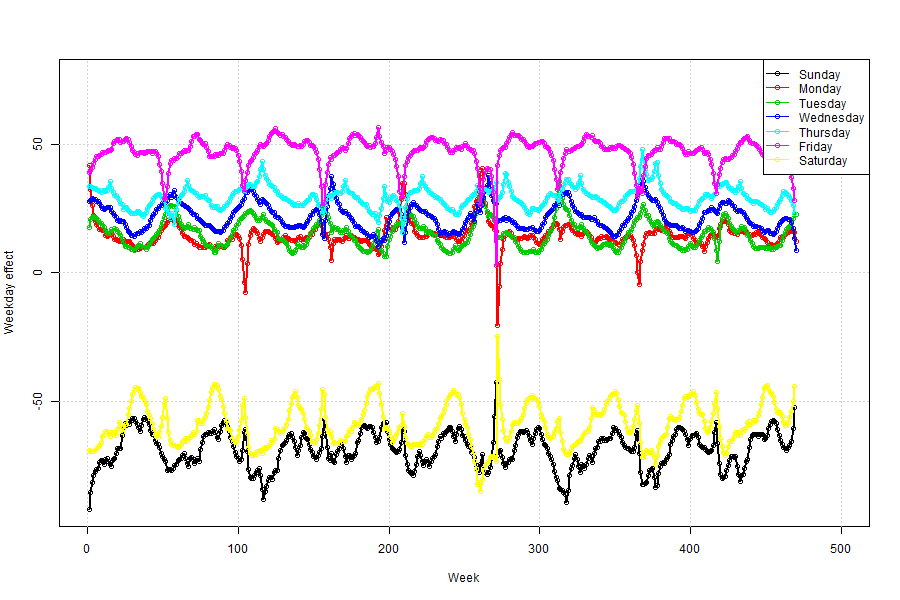
\includegraphics{images/days of the week 2.png}
\caption{alt text}
\end{figure}

    \section{Weekly}\label{weekly}

Spectral analysis from fitting an AR(35) model to the data

\begin{figure}[htbp]
\centering
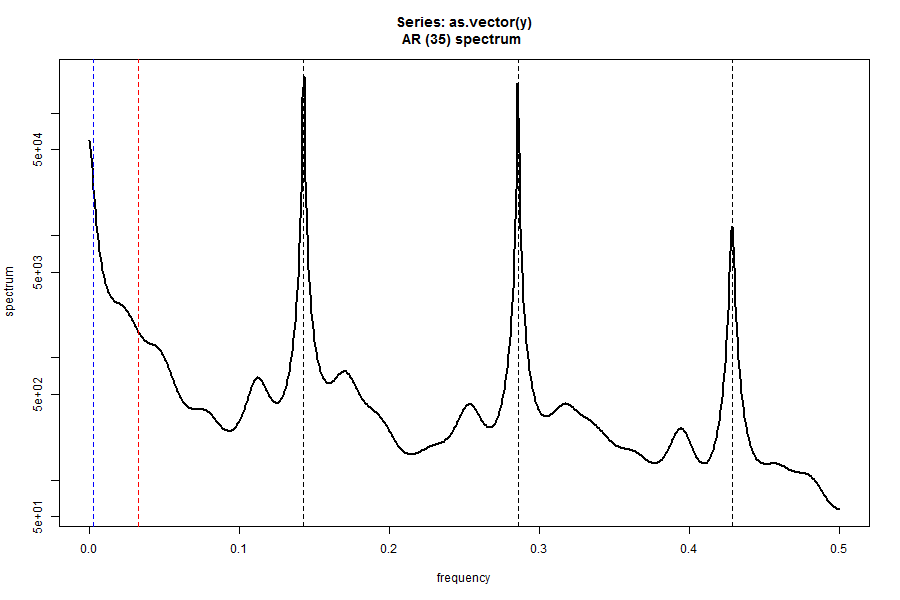
\includegraphics{images/spectral analysis.png}
\caption{alt text}
\end{figure}

    \section{Monthly}\label{monthly}

\begin{figure}[htbp]
\centering
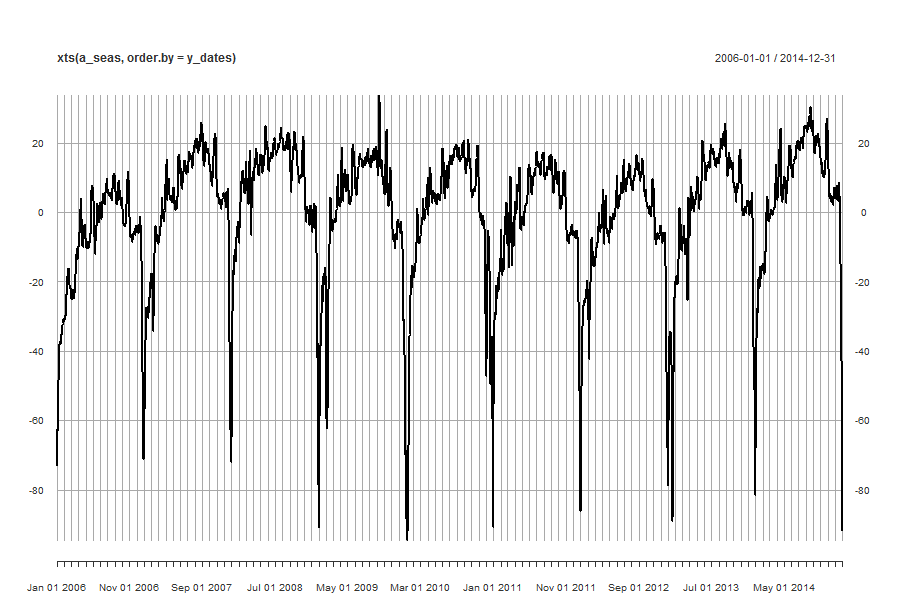
\includegraphics{images/monthly 2.png}
\caption{alt text}
\end{figure}

    \section{Residuals around easter}\label{residuals-around-easter}

    \begin{Verbatim}[commandchars=\\\{\}]
{\color{incolor}In [{\color{incolor}108}]:} \PY{n}{easter\PYZus{}df} \PY{o}{=} \PY{n}{pd}\PY{o}{.}\PY{n}{read\PYZus{}csv}\PY{p}{(}\PY{l+s+s2}{\PYZdq{}}\PY{l+s+si}{\PYZob{}\PYZcb{}}\PY{l+s+s2}{/ts\PYZus{}results/easter\PYZus{}coeff.csv}\PY{l+s+s2}{\PYZdq{}}\PY{o}{.}\PY{n}{format}\PY{p}{(}\PY{n}{os}\PY{o}{.}\PY{n}{getcwd}\PY{p}{(}\PY{p}{)}\PY{p}{)}\PY{p}{,} \PY{n}{index\PYZus{}col} \PY{o}{=} \PY{l+m+mi}{0}\PY{p}{)}
\end{Verbatim}


    \begin{Verbatim}[commandchars=\\\{\}]
{\color{incolor}In [{\color{incolor}109}]:} \PY{n}{easter\PYZus{}df}
\end{Verbatim}


\begin{Verbatim}[commandchars=\\\{\}]
{\color{outcolor}Out[{\color{outcolor}109}]:}             -2    -1     0     1     2
          Easter                                
          16/04/06 -4.97  1.97  0.58 -1.83  2.18
          08/04/07 -4.82  2.16  0.63 -1.70  2.74
          23/03/08 -5.51  1.33 -0.44 -1.27  2.99
          12/04/09 -5.37  1.96  0.18 -1.46  2.44
          04/04/10 -4.99  1.96  0.34 -2.16  2.55
          24/04/11 -5.38  0.63  1.43 -0.54  1.73
          08/04/12 -4.99  2.05  0.11 -2.39  2.84
          31/03/13 -4.73  2.03 -0.39 -2.59  2.21
          20/04/14 -4.56  1.90  0.08 -1.37  2.63
\end{Verbatim}
            
    \section{Significant days}\label{significant-days}

Including the effects of rain and temperature

    \begin{Verbatim}[commandchars=\\\{\}]
{\color{incolor}In [{\color{incolor}110}]:} \PY{n}{days\PYZus{}df} \PY{o}{=} \PY{n}{pd}\PY{o}{.}\PY{n}{read\PYZus{}csv}\PY{p}{(}\PY{l+s+s2}{\PYZdq{}}\PY{l+s+si}{\PYZob{}\PYZcb{}}\PY{l+s+s2}{/ts\PYZus{}results/sig\PYZus{}days.csv}\PY{l+s+s2}{\PYZdq{}}\PY{o}{.}\PY{n}{format}\PY{p}{(}\PY{n}{os}\PY{o}{.}\PY{n}{getcwd}\PY{p}{(}\PY{p}{)}\PY{p}{)}\PY{p}{,} \PY{n}{index\PYZus{}col} \PY{o}{=} \PY{l+m+mi}{0}\PY{p}{)}
\end{Verbatim}


    \begin{Verbatim}[commandchars=\\\{\}]
{\color{incolor}In [{\color{incolor}112}]:} \PY{n}{days\PYZus{}df}\PY{o}{.}\PY{n}{sort\PYZus{}values}\PY{p}{(}\PY{l+s+s2}{\PYZdq{}}\PY{l+s+s2}{Coefficient}\PY{l+s+s2}{\PYZdq{}}\PY{p}{)}
\end{Verbatim}


\begin{Verbatim}[commandchars=\\\{\}]
{\color{outcolor}Out[{\color{outcolor}112}]:}                                                     Coefficient  \textbackslash{}
          Additional Holiday for Wedding of Kate and William      -136.10   
          Christmas Day                                           -113.26   
          New Year Bank Holiday                                   -108.68   
          Good Friday                                             -103.16   
          Late May Bank Holiday                                    -91.11   
          Additional Holiday for Queens Diamond Jubilee            -89.29   
          Christmas Bank Holiday                                   -84.30   
          Early May Bank Holiday                                   -80.01   
          August Bank Holiday (England and Wales)                  -77.27   
          Boxing Day Bank Holiday                                  -70.55   
          Easter Monday                                            -67.69   
          Christmas Eve                                            -35.32   
          Deviation from mean daily rain fall                       -0.40   
          Deviation from mean daily temperature                      0.45   
          
                                                              Standard Error  
          Additional Holiday for Wedding of Kate and William           10.07  
          Christmas Day                                                 5.03  
          New Year Bank Holiday                                         3.67  
          Good Friday                                                   3.36  
          Late May Bank Holiday                                         3.36  
          Additional Holiday for Queens Diamond Jubilee                10.07  
          Christmas Bank Holiday                                        5.05  
          Early May Bank Holiday                                        3.36  
          August Bank Holiday (England and Wales)                       3.35  
          Boxing Day Bank Holiday                                       3.50  
          Easter Monday                                                 3.36  
          Christmas Eve                                                 3.50  
          Deviation from mean daily rain fall                           0.06  
          Deviation from mean daily temperature                         0.13  
\end{Verbatim}
            
    \section{Residuals}\label{residuals}

Even with all of the above, there is still a lot of unexplained
structure in the time series 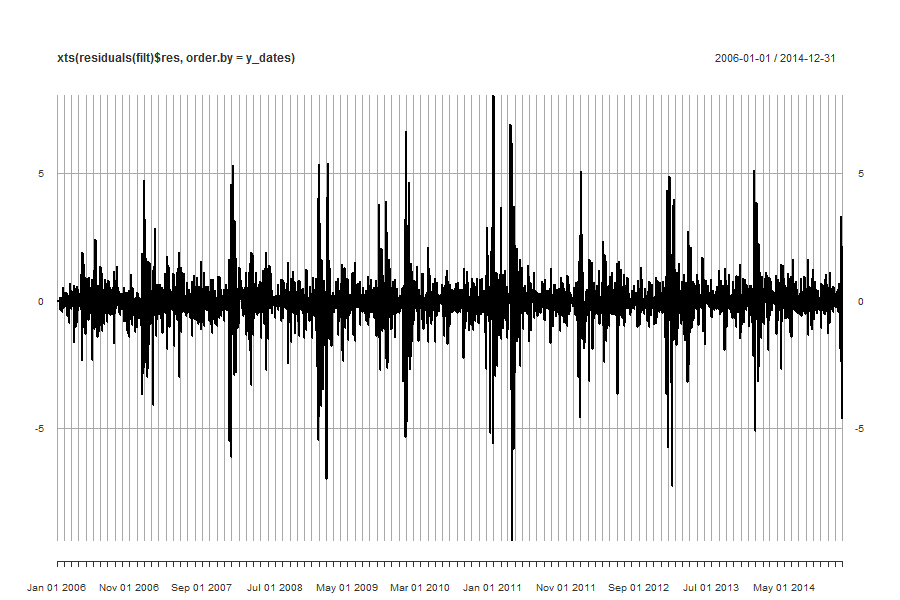
\includegraphics{images/resid 2.png}

    \section{Thank you for listening}\label{thank-you-for-listening}

See these slides again!

Gitpages : https://onsbigdata.github.io/RSS-2018/\\
Github repo: https://github.com/ONSBigData/RSS-2018/

Email: edward.rowland@ons.gov.uk

    \# Data - Traffic flow

    \section{Data - Economic and labour market
measures}\label{data---economic-and-labour-market-measures}

    Annual figures are taken to match with traffic flow

\begin{itemize}
\tightlist
\item
  \textbf{GDP:} The measure used here is the National GDP growth figure
  as contained in the UK National Accounts Blue Book.
\item
  \textbf{CPIH:} The annual UK Consumer Price index including owner
  occupied housing costs is used here. Note that this time series only
  dates to 2005, so no figure is available before this date
\item
  \textbf{CPI:} The annual UK Consumer Price index is used here as CPIH
  is not available before 2005
\item
  \textbf{Unemployment:} The seasonally adjusted UK unemployment rate
  for over 16s is used here
\item
  \textbf{Earnings:} Average weekly earnings is the figure used that
  gives the money paid per week, per job before tax and other deductions
  to employees in the UK
\end{itemize}

    \section{Correlations with annual
measures}\label{correlations-with-annual-measures}

    Pearson's correlations of AADF traffic and economic measures lagged by
one year

    \section{Coefficents}\label{coefficents}

    \paragraph{Department for Transport
data}\label{department-for-transport-data}

\begin{itemize}
\tightlist
\item
  Annual average daily flow (AADF) for major and minor roads is used as
  a measure of traffic flow from 2003 to 2015
\item
  Split into different vehicle categories
\item
  Daily flow is the number of vehicles passing a point on a road on a
  day. This is averaged across the year to produce the average daily
  flow
\item
  This measure is based upon approximate 10,000 manual counts per year,
  between March and October on non-school and public holidays
\item
  These counts are used to estimate AADF figures for major roads
\item
  A representative sample of minor road sites are selected as
  observations points
\item
  These figures are combined with the change on the previous year to
  estimate counts for all minor roads
\end{itemize}

    \begin{verbatim}
<tr>      <th></th>       </tr>    <tr>      <th>Economic indicator</th>      <th>CPI</th>      <th>Change in unemployment (% pts)</th>      <th>Change in weekly earnings (£)</th>      <th>GDP Growth</th>    </tr>    <tr>      <th>Vehicle type</t >      <th></th>      <th></th>      <th></th>      <th></th>    </tr>  </thead>  <tbody>    <tr>      <th>All HGVs</th>      <td>0.08</td>      <td>-0.15</td>      <td>0.95</td>      <td>0.51</td>    </tr>    <tr>      <th>All Motor Vehicles</th>      <td>0.09</td>      <td>-0.50</td>      <td>0.83</td>      <td>0.76</td>    </tr>    <tr>      <th>Buses and Coaches</th>      <td>0.11</td>      <td>-0.56</td>      <td>0.72</td>      <td>0.76</td>    </tr>    <tr>      <th>Cars and Taxis</th>      <td>0.10</td>      <td>-0.46</td>      <td>0.84</td>      <td>0.77</td>    </tr>    <tr>      <th>LGVs</th>      <td>-0.05</td>      <td>-0.67</td>      <td>0.18</td>      <td>0.44</td>    </tr>    <tr>      <th>Motorbikes and Scooters</th>      <td>0.07</td>      <td>0.12</td>      <td>0.83</td>      <td>0.26</td>    </tr>    <tr>      <th>Pedal Cycles</th>      <td>0.04</td>      <td>-0.57</td>      <td>-0.18</td>      <td>0.37</td>    </tr>  </tbody></table>'
\end{verbatim}

    \subsubsection{Stats Netherlands}\label{stats-netherlands}

\begin{longtable}[c]{@{}lcr@{}}
\toprule
Measure & Total Traffic & Cat 1 (\textless{} 5.6m)
Traffic\tabularnewline
\midrule
\endhead
Inflation & -0.42 & -0.43\tabularnewline
Unemployment & -0.47 & -0.41\tabularnewline
Income & 0.74 & 0.74\tabularnewline
GDP & 0.54 & 0.63\tabularnewline
\bottomrule
\end{longtable}

    \section{Time series models}\label{time-series-models}

    \subsubsection{Approach}\label{approach}

\begin{enumerate}
\def\labelenumi{\arabic{enumi}.}
\tightlist
\item
  Try some basic Auto-regressive (AR) models

  \begin{itemize}
  \tightlist
  \item
    These contain one variable, where you are trying to predict future
    values from past (lagged) values
  \item
    These shouldn't work well, otherwise it would be easy to predict GDP
    etc!
  \end{itemize}
\item
  Add in All Vehicles variable in a Vector AR (VAR) model to predict the
  economic variable

  \begin{itemize}
  \tightlist
  \item
    If traffic flow is a good predictor, then this should give a better
    estimate of GDP
  \end{itemize}
\end{enumerate}

    \subsection{Results}\label{results}

    \begin{Verbatim}[commandchars=\\\{\}]
{\color{incolor}In [{\color{incolor}24}]:} \PY{n}{IFrame}\PY{p}{(}\PY{l+s+s2}{\PYZdq{}}\PY{l+s+s2}{figures/actual\PYZus{}vs\PYZus{}AR\PYZus{}predictions.html}\PY{l+s+s2}{\PYZdq{}}\PY{p}{,}
                \PY{n}{width}\PY{o}{=}\PY{l+m+mi}{800}\PY{p}{,} 
                \PY{n}{height}\PY{o}{=}\PY{l+m+mi}{600}
               \PY{p}{)}
\end{Verbatim}


\begin{Verbatim}[commandchars=\\\{\}]
{\color{outcolor}Out[{\color{outcolor}24}]:} <IPython.lib.display.IFrame at 0x7fa2a59d3eb8>
\end{Verbatim}
            
    \section{Caveats}\label{caveats}

    \begin{enumerate}
\def\labelenumi{\arabic{enumi}.}
\tightlist
\item
  Small timeseries
\item
  In-sample predictions
\item
  Recession is an outlier, may be biasing correlations
\item
  Does give some indication that this could work (with better data and
  methods)
\end{enumerate}

    \section{Overall Summary}\label{overall-summary}

    \begin{itemize}
\tightlist
\item
  Weekly earnings, GDP and unemployment look like good candidates, like
  Stats Netherlands
\item
  Though no correlation with inflation
\item
  Evidence that traffic flow can be used as an early indicator for
  economic measures
\item
  Need more data to allow for more sophisticated methods
\end{itemize}

    \section{Daily traffic flow trends}\label{daily-traffic-flow-trends}

Daily traffic flow showing mean 15 min traffic counts averaged across
previous 91 days

    \begin{Verbatim}[commandchars=\\\{\}]
{\color{incolor}In [{\color{incolor}17}]:} \PY{n}{IFrame}\PY{p}{(}\PY{l+s+s2}{\PYZdq{}}\PY{l+s+s2}{figures/quarterly\PYZus{}smoothed\PYZus{}daily\PYZus{}time\PYZus{}series\PYZus{}multi\PYZus{}metrics\PYZus{}small.html}\PY{l+s+s2}{\PYZdq{}}\PY{p}{,}
                \PY{n}{width}\PY{o}{=}\PY{l+m+mi}{800}\PY{p}{,} 
                \PY{n}{height}\PY{o}{=}\PY{l+m+mi}{600}
               \PY{p}{)}
\end{Verbatim}


\begin{Verbatim}[commandchars=\\\{\}]
{\color{outcolor}Out[{\color{outcolor}17}]:} <IPython.lib.display.IFrame at 0x7f69e0bdf128>
\end{Verbatim}
            
    \section{Annual components of traffic flow
data}\label{annual-components-of-traffic-flow-data}

    \subsubsection{Trends}\label{trends}

    \begin{Verbatim}[commandchars=\\\{\}]
{\color{incolor}In [{\color{incolor}19}]:} \PY{n}{IFrame}\PY{p}{(}\PY{l+s+s2}{\PYZdq{}}\PY{l+s+s2}{figures/trends\PYZus{}traffic\PYZus{}flow\PYZus{}decomposition.html}\PY{l+s+s2}{\PYZdq{}}\PY{p}{,}
                \PY{n}{width}\PY{o}{=}\PY{l+m+mi}{800}\PY{p}{,} 
                \PY{n}{height}\PY{o}{=}\PY{l+m+mi}{400}
               \PY{p}{)}
\end{Verbatim}


\begin{Verbatim}[commandchars=\\\{\}]
{\color{outcolor}Out[{\color{outcolor}19}]:} <IPython.lib.display.IFrame at 0x7f69e0bdf3c8>
\end{Verbatim}
            
    \section{Yearly component}\label{yearly-component}

    \begin{Verbatim}[commandchars=\\\{\}]
{\color{incolor}In [{\color{incolor}21}]:} \PY{n}{IFrame}\PY{p}{(}\PY{l+s+s2}{\PYZdq{}}\PY{l+s+s2}{figures/seasons\PYZus{}trends\PYZus{}traffic\PYZus{}flow\PYZus{}decomposition.html}\PY{l+s+s2}{\PYZdq{}}\PY{p}{,}
                \PY{n}{width}\PY{o}{=}\PY{l+m+mi}{800}\PY{p}{,} 
                \PY{n}{height}\PY{o}{=}\PY{l+m+mi}{400}\PY{err}{`}
               \PY{p}{)}
\end{Verbatim}


\begin{Verbatim}[commandchars=\\\{\}]
{\color{outcolor}Out[{\color{outcolor}21}]:} <IPython.lib.display.IFrame at 0x7f69e0bdf278>
\end{Verbatim}
            
    \subsubsection{Residuals}\label{residuals}

    \begin{Verbatim}[commandchars=\\\{\}]
{\color{incolor}In [{\color{incolor}23}]:} \PY{n}{IFrame}\PY{p}{(}\PY{l+s+s2}{\PYZdq{}}\PY{l+s+s2}{figures/resids\PYZus{}trends\PYZus{}traffic\PYZus{}flow\PYZus{}decomposition.html}\PY{l+s+s2}{\PYZdq{}}\PY{p}{,}
                \PY{n}{width}\PY{o}{=}\PY{l+m+mi}{800}\PY{p}{,} 
                \PY{n}{height}\PY{o}{=}\PY{l+m+mi}{400}
               \PY{p}{)}
\end{Verbatim}


\begin{Verbatim}[commandchars=\\\{\}]
{\color{outcolor}Out[{\color{outcolor}23}]:} <IPython.lib.display.IFrame at 0x7f69e0bdf780>
\end{Verbatim}
            

    % Add a bibliography block to the postdoc
    
    
    
    \end{document}
